\section{Evaluation}\label{sec:evaluation}
We now present the results of our experimental analysis to evaluate the SEU protection approach. We first introduce three test applications with different degrees of stack dynamism to evaluate the protection efficacy of our approach. We then validate the correctness of our approach, and analyze the relationship between the successful SEU protection probability and the SEU injection rate. Finally, we consider the overhead introduced by our approach, both interms of space and execution speed. Ubuntu 13.10, with Linux kernel version 3.8, and GCC 4.1.2 are used throughout.

\begin{comment}
\subsection{SEU Simulation Library}
To evaluate our approach, we implemented a library to retrieve the current stack range, and to simulate SEUs by randomly flipping bits in the stack. The library includes a timer that fires at a configurable rate, and a corresponding interrupt handler which performs the following two tasks. 

(i) The interrupt handler calculates the stack range and size, excluding the stack frame of the interrupt handler itself. This is achieved by reading the stack pointer, SP; the lowest stack address is specified by the\textit{RAM\_END} constant. Since the number of registers used by the interrupt handler can be easily determined, the size of the handler's stack frame is known, --- 24 bytes. The top stack address is $SP + 24$. The stack size is $RAM\_END - SP - 24$. The stack range is from \textit{RAM\_END} to $SP + 24$. The value of the stack pointer is sent to a desktop via UART for analysis purposes.

(ii) The interrupt handler generates an SEU randomly, simulating an SEU caused by a high-energy particle. In thefirst version of the design, the standard random number generation function provided by \textit{avr-libc} library~\cite{avrlibc} was used, with the system clock counter providing the seed(s). However, identical sequences of random numbers were generated by the function because of xxx. In the second version of the design, a large sequence of random numbers was generated on a desktop, and was then written to the program memory of the microprcessor. However, the random number sequence took too much program memory (e.g., 30 KB). In our final version of the design, ADC readings were used as random seeds, with the standard random number generator. An ADC pin (PA0) was left to \textit{floating}, and its readings are used as seeds.
\end{comment}

\subsection{Test Applications}

To evaluate our approach under varying stack conditions and SEU frequencies, three AVR applications are introduced. The stack usage pattern of each application is shown in Figure \ref{fig:stacksize_usage}. The x-axis represents execution time, and the y-axis represents stack size. Below is a description of each application.

\begin{itemize}
\item The \textbf{Delay} application repeatedly executes a function that contains a delay of 4400 clock cycles, implemented using a while loop, yielding low stack variability.
\item The \textbf{Double Function Calls} application repeatedly executes three functions --- function A calls B, and function B calls C --- yielding moderate stack variability.
\item The \textbf{Fibonacci} application repeatedly calculates the tenth Fibonacci number using recursion, yielding significant stack variability.
\end{itemize}

\begin{figure}[H]
\centering
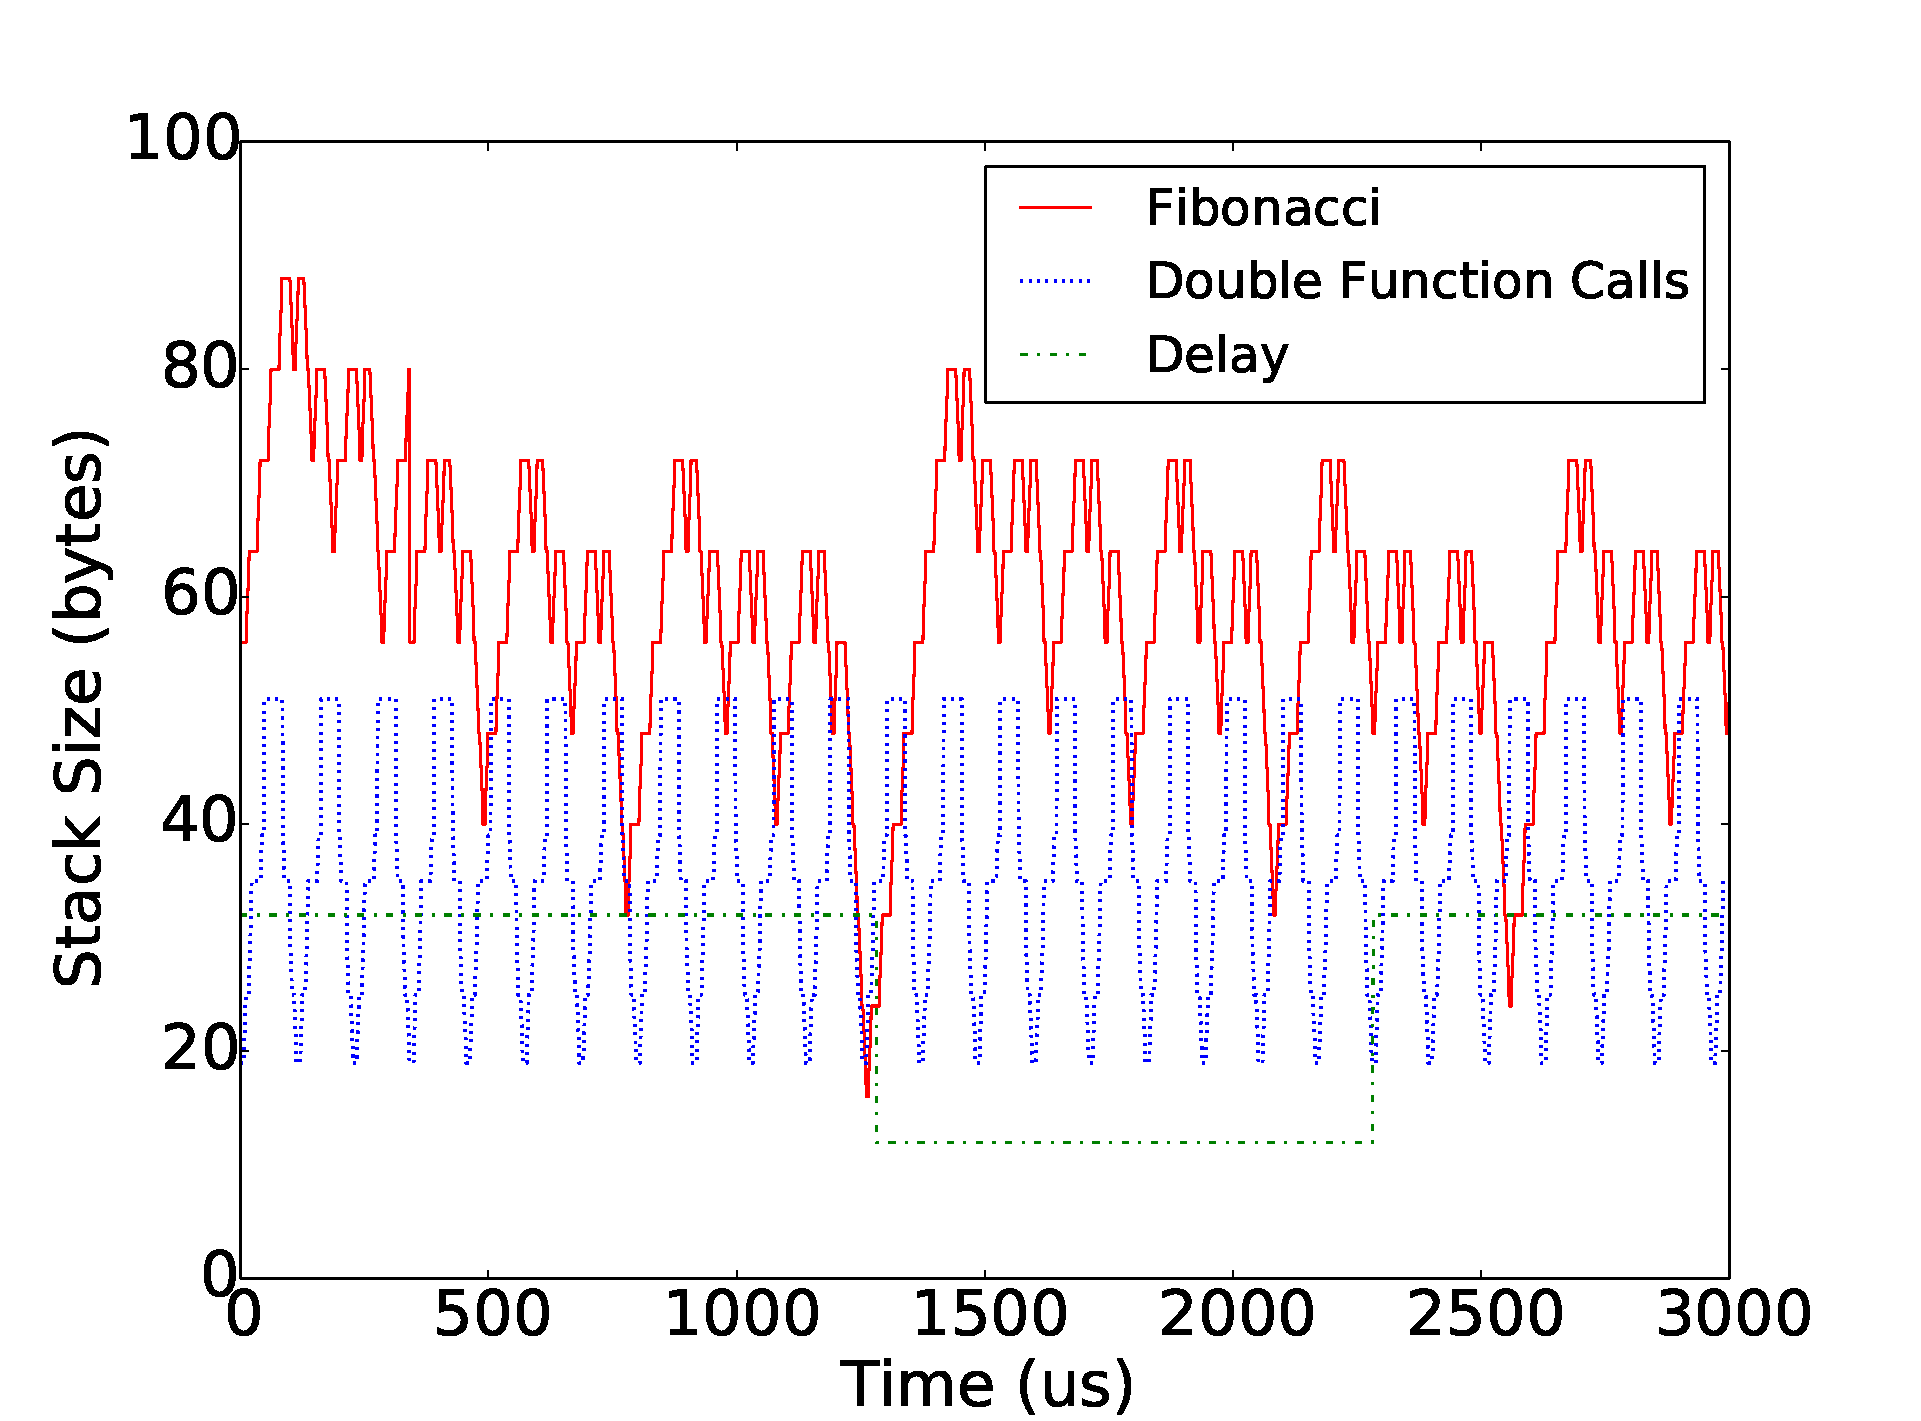
\includegraphics[width=0.5\textwidth]{figures/stacksize_usage_v3.pdf}
\caption{Stack Usage of Test Applications}
\label{fig:stacksize_usage}
\end{figure}

\subsection{Validation}

We first validate our approach and consider the SEU protection efficacy it affords. We focus our analysis on stack frame protection. 

We first assume that the stack frame of the currently-executing function is not affected by SEUs. We use induction to prove the correctness of our approach. Suppose the current stack contains $n$ stack frames. If $n=1$, the currently-executing function is the \textit{main} function. It will not be affected according to the assumption. Assume the stack is protected when $n=k\enspace(k\geq2)$. Now consider when $n=k-1$. Since the currently-executing function's stack frame, the ($k-1$)th stack frame, is protected by it's callee, when the callee returns, the ($k-1$)th stack frame is guaranteed to be correct. Since the current stack frame is not affected according to the assumption, the stack is protected when $n=k-1\enspace (n\geq2)$. By induction, the stack is protected when the current stack frame is not affected.%Now consider when $n=k+1 (k\geq2)$. The stack frame of the current function's caller is not affected before the current function starts executing. When the current function starts executing, its stack frame is established, and the stack frame is not affected according to the assumption. So the stack is protected when $n=k+1 (n\geq2)$. By induction, the stack is protected when the current stack frame is not affected.
%When the function returns, it checks if its caller's stack frame is affected and restores the caller's stack frame if it is. This process continues throughout the life cycle of the program. Each function, except the \textit{main} function, protects its caller from being affected by an SEU. we claim that our approach protects the stack from SEUs, excluding current function's stack frame. 

To verify this claim, the AVR Simulator IDE~\cite{avrsimide} was used to manually inject SEUs and observe the execution results. The results show that each function is able to detect and fix SEUs introduced ``beneath'' the topmost stack frame.

However, if the stack frame of the current function is affected by an SEU, protection is not guaranteed. If the SEU changes key data, such as the return address or stack frame size, the current function will not execute as expected. We assume that only one SEU will occur during a given function execution, and that the SEU is uniformly likely to affect all bits in RAM. The probability of successful SEU protection can be expressed as:
\begin{equation}\label{eq_seu1}
p=1-\frac{c}{s+e}
\end{equation}
Where $p$ is the probability of successful protection, $c$ is the size of the current stack frame, $s$ is the size of the stack, and $e$ is the size of the unused space between the heap and the stack.

We extend our analysis to cases where more than one SEU may occur during a given function execution. The probability of successful SEU protection can be expressed as:
\begin{equation}\label{eq_seu2}
\begin{split}
&p=(1-\frac{c}{s+e})^n\{(1-\frac{6}{s+e-c})^n \\
&+\mathrm{C}_3^2(1-\frac{4}{s+e-c})^n[1-(1-\frac{2}{s+e-c-4})^n]\}
\end{split}
\end{equation}
Where $p$ is the probability of success, $c$ is the size of the current stack frame, $s$ is the size of the stack, $e$ is the size of the unused space between the heap and the stack, and $n$ is the number of SEUs that occur during the function's execution. Our approach succeeds when the currently-executing function's stack frame is not affected and at most one of three copies of the caller's stack frame size is affected. In equation \ref{eq_seu2}, $(1-\frac{c}{s+e})^n$ is the probability that the currently-executing function's stack frame is not affected. $(1-\frac{6}{s+e-c})^n$ is the probability that all the three copies of the caller's stack frame are not affected. $\mathrm{C}_3^2(1-\frac{4}{s+e-c})^n[1-(1-\frac{2}{s+e-c-4})^n]$ is the probability that any two of the three copies are not affected, regardless of the other one. The component within the braces is the probability that at most one copy is affected.%Equation \ref{eq_seu2} represents the probability that the current stack frame is affected and at most one of the three copies of the caller's stack frame size is affected. The protection process does not work if it cannot retrieve the correct stack frame size for the calling function; the size is needed for CRC calculation and frame copy.

In equation \ref{eq_seu2}, the number of SEUs that occur, $n$, can be expressed as:
\begin{equation}
n = \frac{y*l}{m}*f
\end{equation}
where $y$ is the number of clock cycles used to execute an instruction, $m$ is the frequency of the microprocessor, $l$ is the number of instructions in the current function, and $f$ is the rate at which SEUs are injected in RAM. In our configuration, most AVR instructions cost 2 clock cycles to execute, and the frequency of our ATmega644 is set to 10MHz.

\begin{table}
	\center
    \begin{tabular}{|l|c|c|c|c|}
    \hline
    \textbf{ Applications}   & \textbf{l} & \textbf{c} & \textbf{s} & \textbf{e}	\\ \hline
    Delay         				& 115			& 16		& 30		& 3022		\\ \hline
    Double Function Calls       & 54			& 9			& 30        & 3022		\\ \hline
    Fibonacci             		& 42			& 10		& 60	   	& 2992		\\ \hline
    \end{tabular}
    \caption {Applications Stack Characteristic}
    \label{tbl_application_parameters}
\end{table}
\begin{figure}
\centering
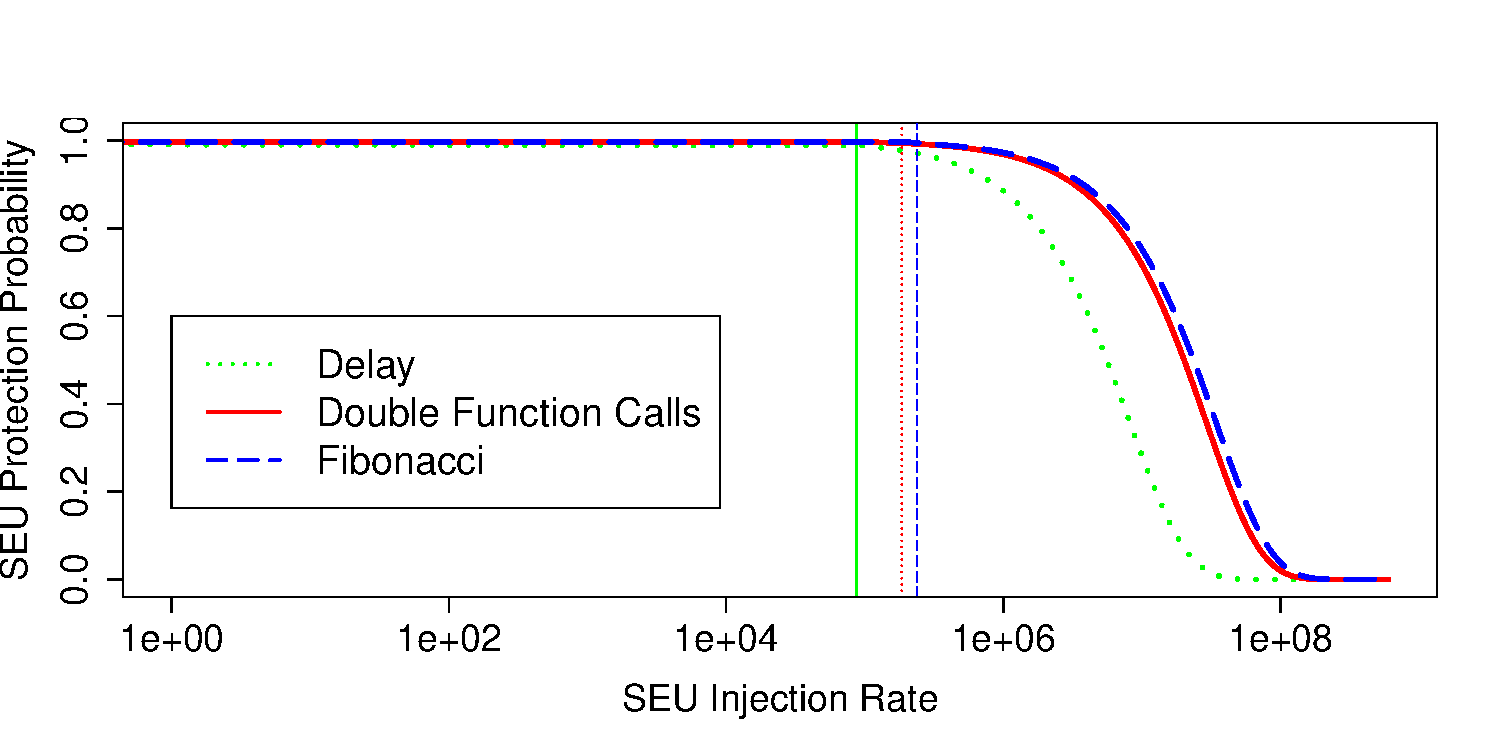
\includegraphics[width=0.5\textwidth]{figures/success_probability_v1.pdf}
\caption{Successful SEU Protection Probability}
\label{fig:success_probability}
\end{figure}
We now consider the relationship between the successful SEU protection probability and the SEU occurrence rate. To demonstrate the relationship, we collect the corresponding parameters of the three test applications using AVR Simulator IDE, as shown in Table \ref{tbl_application_parameters}. Figure \ref{fig:success_probability} plots the change in successful SEU protection probability as a function of SEU injection frequency. The x-axis denotes the rate at which SEUs are injected, and the y-axis denotes successful SEU protection probability. Each vertical line shows where the number of SEUs begins to exceed 1 (for each application). For each application, when only one SEU occurs during a given function execution (left side of the vertical line), the successful SEU protection probability is constant (Delay: 99.48\%, Double Function Calls: 99.71\%, Fibonacci: 99.67\%), because the only case the approach cannot handle is when the current frame is affected. When more than one SEU occurs during a given function execution (right side of the vertical line), the successful SEU protection probability increases because the SEUs may affect both the stack frame of the current function and the stack frame size of the caller stored in the stack. As the SEU occurrence rate increases, the successful SEU protection probability decreases, until it approaches 0. The lower the stack dynamism, the longer the function execution time, which increases the probability of SEU occurrence in the current stack frame. Low stack frame dynamism causes successful SEU protection probability of Delay drop significantly before the other two applications, as shown in Figure \ref{fig:success_probability}.

\subsection{Performance}
Since the same code is injected for every function, the execution overhead is similar for all functions, varying only when an SEU is detected. Table \ref{tbl_speed_overhead} summarizes the overhead of each injected code segment. The second column lists the number of times each code segment executes (per function), the third column lists the number of instructions executed in each code segment, the fourth column lists the number of clock cycles spent executing each code segment, and the fifth column lists the ROM space overhead for each injected segment. $S$ denotes the size of the recovered stack frame. The \textit{CRC Calculation} code segment and \textit{STP Update} code segment execute twice for each function, and the \textit{frame copy} code segment executes either once or twice, depending on whether an SEU is detected. Each of the other code segments executes once for each function. Therefore, the minimum overhead introduced in terms of number of clock cycles is $62*S+304$, when no SEU is detected. The worst case is $70*S+432$ clock cycles, when an SEU is detected. 
\begin{table*}
	\center
    \begin{tabular}{|l|c|c|c|c|}
    \hline
   \textbf{ Code Segment}   & \textbf{Number of Execution} & \textbf{Instructions} & \textbf{Clock Cycles} & \textbf{ROM Space}	\\ \hline
    CRC Calculation         & 2			& 24*S+1		& 27*S+4		& 50				\\ \hline
    CRC Save                & 1			& 13			& 26           	& 26				\\ \hline
    CRC Compare             & 1			& 27			& 52		   	& 64				\\ \hline
    Frame Copy				& 1 or 2	& 64+4*S		& 8*S+128      	& 50				\\ \hline
%    Frame Copy (Worst Case) & 1 		& 73+4*S      & 144+8*S      & 50				\\ \hline
    Frame Size save         & 1			& 18			& 34           	& 36				\\ \hline
    STP Initialization		& 1			& 16			& 28		   	& 32				\\ \hline
	STP Update				& 2			& 7				& 14			& 14				\\ \hline
	\textbf{Total (No Recovery)} & -	 	& 48*S+154     	& 62*S+304		& 272  		\\ \hline
	\textbf{Total (Recovery)}& -	 		& 52*S+218     	& 70*S+432		& 272 		\\ \hline
    \end{tabular}
    \caption {Speed Overhead}
    \label{tbl_speed_overhead}
\end{table*}

We next evaluate space overhead using the three test applications. The ROM space data was collected using $avr-size$. The results are summarized in Figure \ref{fig:space_overhead}. The y-axis denotes the ROM space overhead, in bytes. Delay and Fibonacci involve two functions, and Double Function Calls involves four. From Figure \ref{fig:space_overhead}, we can see that the ROM overhead of the Double Function Calls application is twice the Delay and Fibonacci applications. The ROM overhead is related only to the number of functions in the program.
\begin{figure}
\centering
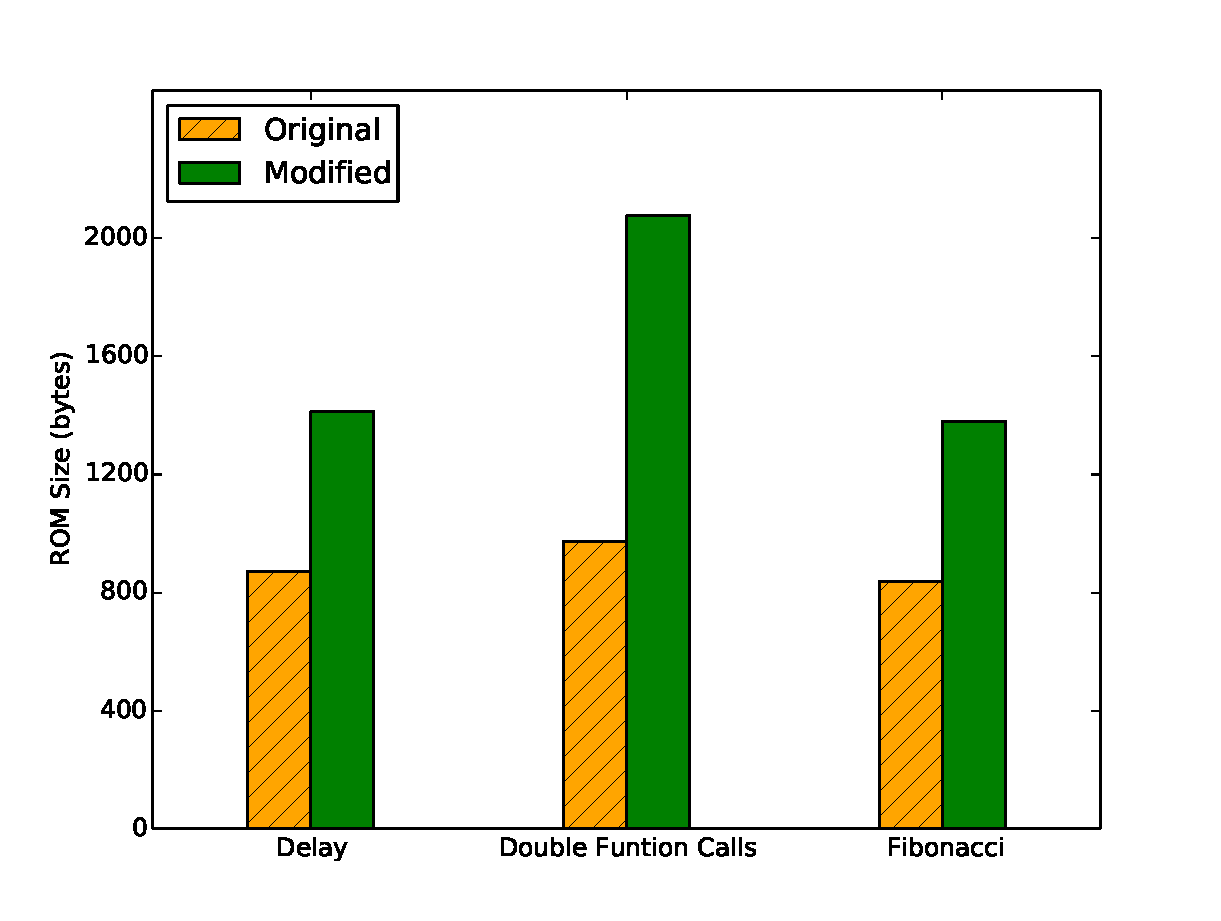
\includegraphics[width=0.5\textwidth]{figures/space_overhead.pdf}
\caption{Space Overhead}
\label{fig:space_overhead}
\end{figure}
We next evaluate execution speed overhead. The execution time is obtained using AVR Simulator IDE. The results are summarized in Figure \ref{fig:speed_overhead}. The y-axis represents the execution time, obtained using AVR Simulator IDE. Each \textit{Original} bar shows the execution time of the original application; each \textit{No Recovery} bar shows the execution time of the protected application with no SEUs detected; each \textit{Recovery} bar shows the execution time of the protected application with SEUs detected. The figure shows that the stack variability impacts the speed overhead. The greater the stack dynamism, the greater the speed overhead. The explanation is that high stack dynamism shows dense function invocation, and indicates high execution speed overhead caused by the injected code.
\begin{figure}
\centering
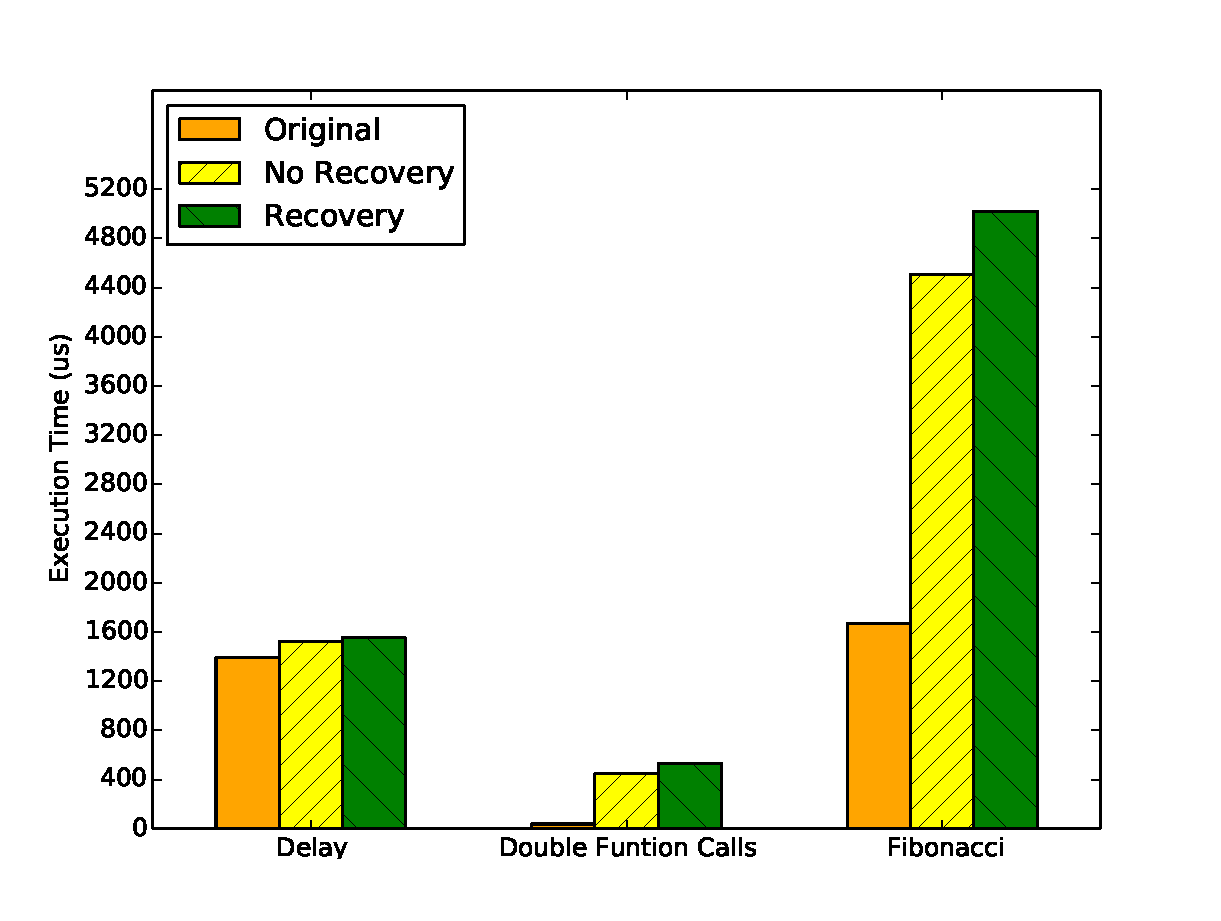
\includegraphics[scale=0.4]{figures/speed_overhead.pdf}
\caption{Speed Overhead}
\label{fig:speed_overhead}
\end{figure}